\documentclass{article}
\usepackage{graphicx}
\usepackage[dvipsnames,table]{xcolor}
\usepackage[utf8]{inputenc}
\usepackage{siunitx}
\usepackage[american,siunitx]{circuitikz}
\usepackage{amsmath}
\usepackage{svg}
\usepackage{booktabs}
\usepackage{float}
\usepackage{xparse, xfp}
\usepackage{multirow}
\usepackage{tikz}
\usepackage{karnaugh-map}
\usepackage{pdfpages}
\usepackage{hyperref}
\hypersetup{
    colorlinks=true,
    linkcolor=blue,
    filecolor=magenta,      
    urlcolor=cyan,
}
\usepackage{caption} 

\makeatletter
\ctikzset{lx/.code args={#1 and #2}{ 
  \pgfkeys{/tikz/circuitikz/bipole/label/name=\parbox{1cm}{\centering #1  \\ #2}}
    \ctikzsetvalof{bipole/label/unit}{}
    \ifpgf@circ@siunitx 
        \pgf@circ@handleSI{#2}
        \ifpgf@circ@siunitx@res 
            \edef\pgf@temp{\pgf@circ@handleSI@val}
            \pgfkeyslet{/tikz/circuitikz/bipole/label/name}{\pgf@temp}
            \edef\pgf@temp{\pgf@circ@handleSI@unit}
            \pgfkeyslet{/tikz/circuitikz/bipole/label/unit}{\pgf@temp}
        \else
        \fi
    \else
    \fi
}}

\ctikzset{lx^/.style args={#1 and #2}{ 
    lx=#2 and #1,
    \circuitikzbasekey/bipole/label/position=90 } 
}

\ctikzset{lx_/.style args={#1 and #2}{ 
    lx=#1 and #2,
    \circuitikzbasekey/bipole/label/position=-90 } 
}
\makeatother

\captionsetup[table]{skip=10pt}

\usetikzlibrary{calc}
%\usepackage[landscape]{geometry}
\renewcommand{\thesubsection}{\thesection.\alph{subsection}}
\newcommand{\equal}{=}
\newcommand{\greyrule}{\arrayrulecolor{black!30}\midrule\arrayrulecolor{black}}
\makeatletter
\newcommand\currcoor{\the\tikz@lastxsaved,\the\tikz@lastysaved}
\makeatother
\newcolumntype{:}{@{\hskip\tabcolsep\color{black!30}\vrule\hskip\tabcolsep}}

\ExplSyntaxOn
\NewExpandableDocumentCommand \groupify { O{\,\allowbreak} m m }
  { \jakob_groupify:nnn {#1} {#2} {#3} }
\cs_new:Npn \jakob_groupify:nnn #1 #2 #3
  { \__jakob_groupify_loop:nnw { 1 } {#2} #3 \q_recursion_tail {#1} \q_recursion_stop }
\cs_new:Npn \__jakob_groupify_loop:nnw #1 #2 #3
  {
    \quark_if_recursion_tail_stop:n {#3}
    \exp_not:n {#3}
    \int_compare:nNnTF {#1} = {#2}
      { \__jakob_groupify_sep:n }
      { \exp_args:Nf \__jakob_groupify_loop:nnw { \int_eval:n { #1+1 } } }
          {#2}
  }
\cs_new:Npn \__jakob_groupify_sep:n #1 #2 \q_recursion_tail #3
  {
    \tl_if_empty:nF {#2} { \exp_not:n {#3} }
    \__jakob_groupify_loop:nnw { 1 } {#1}
    #2 \q_recursion_tail {#3}
  }
\ExplSyntaxOff

\title{ECE 2200L\\Introduction to Microelectronics Circuits Laboratory\\\,\\Experiment 8\\MOSFET Biasing Stability and Signaling\\\,\\Report}
\author{Choi Tim Antony Yung}
\date{November 4, 2020}
\begin{document}
\maketitle

\thispagestyle{empty}
\setcounter{page}{0}

\newpage

\section*{Objective}
To design a 4-resistor biasing circuit to meet specification with a pre existing MOSFET from the earlier Lab (Lab7). 

\section*{Prelab}
\begin{figure}[H]
  \centering
  \begin{circuitikz}
    \draw
    node[nigfete](mos){}
    (mos.D) node[circ]{} node[right]{D} to [R,l_=$R_D$, i<=$I_D$] ++(0,2) coordinate(vcc) node[vcc]{\SI{22}{\volt}}
    (vcc) -- ++(-2,0) to[R=\SI{220}{\kilo\ohm}] (\currcoor|-mos.G) coordinate(mosG) to[short] (mos.G)  node[circ]{} node[above]{G}
    (mos.S) node[circ]{} node[right]{S} to[R=$R_S$] ++(0,-2) node[ground](gnd){}
    (mosG) to[R=\SI{100}{\kilo\ohm}] (\currcoor |- gnd) -- (gnd)
    ;
  \end{circuitikz}
  \caption{Circuit of Step 1 and Step 2}
  \label{fig:ckt1}
\end{figure}

Given $V_T=\SI{1.6}{V}$ and $K_n=0.1\text{\;mAV}^{-2}$, we can determine the value of $R_D$ and $R_S$ such that the circuit is biased to a Q-point of $I_{Dq} = \SI{2.5}{\milli\ampere}$ and $V_{DSq} = \SI{8}{\volt}$
\begin{align}\label{eqn:ckt1}
  V_G &= (\SI{22}{\volt})\frac{100000}{220000+100000}=\SI{6.875}{\volt}\\
  I_D &= \frac{K_n}{2}\left(V_{GS}-V_T\right)^2\\
  2.5 &= \frac{0.1}{2}\left(V_{GS}-1.6\right)^2\\
  V_{GS} &= \SI{1.758}{\volt}\\
  V_S &= V_G - V_{GS} = \SI{5.117}{\volt}\\
  R_S &= \frac{\SI{5.117}{V}}{\SI{2.5}{\milli\ampere}} = \SI{2.05}{\kilo\ohm} \approx \SI{2.2}{\kilo\ohm}\\
  R_D &= \frac{22-V_D}{I_D} = \frac{\left(22-(8+5.117)\right)\text{V}}{\SI{2.5}{\milli\ampere}} = \frac{\SI{8.885}{\volt}}{\SI{2.5}{\milli\ampere}}=\SI{3.553}{\kilo\ohm}\approx\SI{3.9}{\kilo\ohm}
\end{align}

\section*{Procedure}
\subsubsection*{Step 1}
Circuit in figure \ref{fig:ckt1} was constructed with MOSFET with $V_T=\SI{1.6}{V}$ and $K_n=0.1\text{\;mAV}^{-2}$. $V_D$, $V_G$ and $V_S$ was measured in order to determine Q-point parameter $I_{Dq}$ and $V_{DSq}$.

\begin{align*}
  V_D &= \SI{13.00}{\volt}\\
  V_G &= \SI{6.8}{\volt}\\
  V_S &= \SI{5.01}{\volt}
\end{align*}

From the above values $I_{Dq}$ and $V_{DSq}$ can be found

\begin{align*}
  V_{DSq} &= 13.00-5.01=\SI{7.99}{\volt}\text{, a -0.125\% difference from specification}\\
  I_{Dq}  &= \frac{22-13.00}{3900} = \SI{2.3}{\milli\ampere}\text{, a -8\% difference from specification}
\end{align*}

\subsubsection*{Step 2}
Circuit \ref{fig:ckt1} was then constructed with a ddifferent MOSFET. $V_D$, $V_G$ and $V_S$ was measured in order to determine Q-point parameter $I_{Dq}$ and $V_{DSq}$.

\begin{align*}
  V_D &= \SI{12.67}{\volt}\\
  V_G &= \SI{6.8}{\volt}\\
  V_S &= \SI{5.2}{\volt}
\end{align*}

From the above values $I_{Dq}$ and $V_{DSq}$ can be found

\begin{align*}
  V_{DSq} &= 12.67-5.2=\SI{7.47}{\volt}\text{, a -6.51\% difference from }\\
  I_{Dq}  &= \frac{22-12.67}{3900} = \SI{2.39}{\milli\ampere}\text{, a 3.91\% difference from specification}
\end{align*}

\newpage

\subsubsection*{Step 3}

\begin{figure}[H]
  \centering
  \begin{circuitikz}
    \draw
    node[nigfete](mos){}
    (mos.D) node[circ](D){} node[below left]{D} to [R,l_=$R_D$, i<=$I_D$] ++(0,2) coordinate(vcc) node[vcc]{\SI{22}{\volt}}
    (vcc) -- ++(-2,0) to[R,lx_={R$_1$ and \SI{220}{\kilo\ohm}}] (\currcoor|-mos.G) coordinate(G) to[short] (mos.G)  node[circ]{} node[above]{G}
    (mos.S) node[circ]{} node[left](S){S} to[R,l_=$R_S$] ++(0,-2) node[ground](gnd){}
    (G) to[R,lx_={R$_2$ and \SI{100}{\kilo\ohm}}] (\currcoor |- gnd) -- (gnd)
    (S) -- ++(1,0) to[eC=\SI{47}{\micro\farad}] (\currcoor |- gnd)
    (D) to[eC=\SI{0.1}{\micro\farad}] ++(2.5,0) coordinate (Vo) to[R,lx^={\SI{100}{\kilo\ohm}} and R$_\text{L}$] (\currcoor |- gnd) -- (gnd)
    (Vo) -- ++(0.5,0) node[circ]{} node[right]{$V_O$}
    (G) to[eC,l_=\SI{0.1}{\micro\farad}] ++(-2,0) to[sV_=\SI{1}{\kilo\hertz}\;\SI{200}{\milli\volt}$_{\text{pp}}$] (\currcoor|-gnd) -- (gnd)
    ;
  \end{circuitikz}
  \caption{Circuit of Step 3}
  \label{fig:ckt2}
\end{figure}

Given $V_T=\SI{1.6}{V}$ and $K_n=0.1\text{\;mAV}^{-2}$ and a Q-point at $I_{Dq} = \SI{2.5}{\milli\ampere}$ and $V_{DSq} = \SI{8}{\volt}$, we can calculate the small signal transconductance $g_m$ as follow
\begin{align*}
  I_D &= \frac{K_n}{2}\left(V_{GS}-V_T\right)^2\\
  \sqrt{\frac{2}{K_n}I_D}&=\left(V_{GS}-V_T\right)\\
  g_m &= \frac{\delta I_D}{\delta V_{GS}} = K_n\left(V_{GS}-V_T\right)=\sqrt{2K_nI_{Dq}} = \SI{22.36}{\milli\siemens} 
 \end{align*}

 \begin{figure}[H]
  \centering
  \begin{circuitikz}
    \draw[color=blue]
    (0,0) to[cisource,i>_=$g_mV_{gs}$] (0,-2) -- ++(-1,0) coordinate (com) -- ++(-1,0) to[open, v^<=$V_{gs}$] ++(0,2) -- ++(-1,0) node[circ](g){} node[above]{g}
    (0,0) -- ++(1,0) node[circ](d){} node[above]{d}
    (com) -- ++(0,-0.5) node[circ](s){} node[right]{s} node[ground]{}
    ;
    \draw[color=black]
    (d) -- ++(0.75,0) coordinate (RD) -- ++(1.25,0) node[circ]{} node[above]{$V_o$} to[R=$R_L$] ++(0,-2) node[ground]{}
    (RD)  to[R=$R_D$] ++(0,-2) node[ground]{}
    (g) -- ++(-0.75,0) coordinate (R2) -- ++(-1.25,0) coordinate (R1) -- ++(-1.25,0) node[circ]{} node[above]{$V_i$} to[sV=\;] ++(0,-2) node[ground]{}
    (R2)  to[R=$R_2$] ++(0,-2) node[ground]{}
    (R1)  to[R=$R_1$] ++(0,-2) node[ground]{}
    ;
  \end{circuitikz}
  \caption{Circuit in Step 3 using small signal model MOSFET (blue)}
  \label{fig:ckt2smallsig}
\end{figure}

Using the small signal model, $A_V = \frac{V_o}{V_i}$ can then be derived
\begin{align*}
  V_i &= V_{gs}\\
  V_o &= -g_mV_{gs}\left(R_D||R_L \right)\\
  A_V &= \frac{V_o}{V_i} = -g_m\left(R_D||R_L \right)\\
  A_V &= -(\SI{22.36}{\milli\siemens})(\SI{3.9}{\kilo\ohm}||\SI{100}{\kilo\ohm})=-83.93
\end{align*}

\begin{figure}[H]
  \centering
  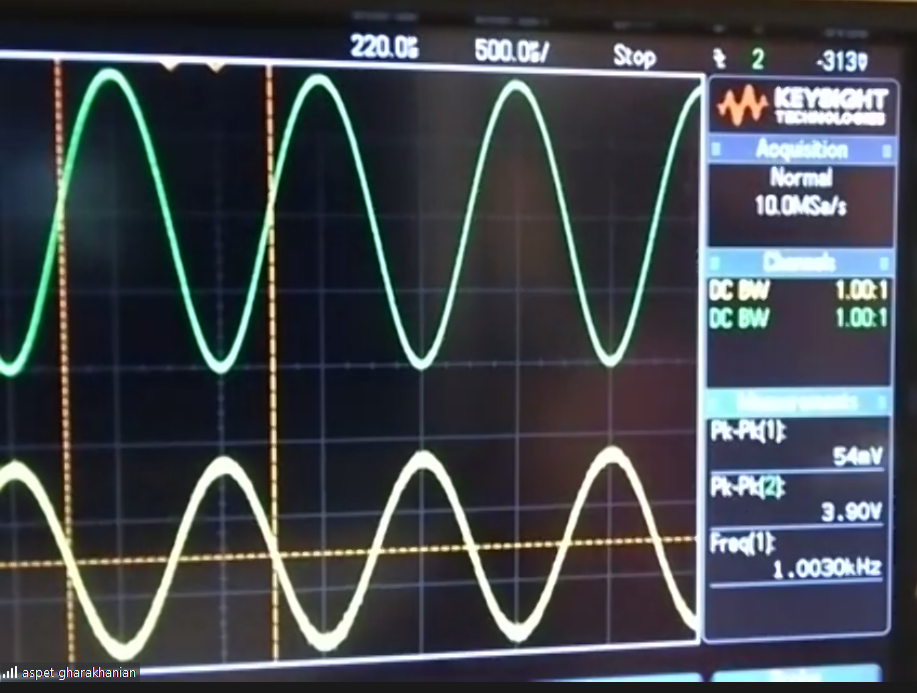
\includegraphics[width=\textwidth]{ECE2200L_Lab8_scope.png}
  \caption{Oscilloscope output of Step 3 circuit (Figure \ref{fig:ckt2}) showing $V_{i_{pp}} = \SI{54}{\milli\volt}$ and $V_{o_{pp}} = \SI{3.90}{\volt}$}
  \label{fig:IV2}
\end{figure}

From the Oscilloscope the experimental value of $A_V$ can be calculated

$$A_V = -\frac{3900}{54}\approx-72.22\text{, a -14.0\% difference from theoretical value}$$

\newpage

\begin{figure}[H]
  \centering
  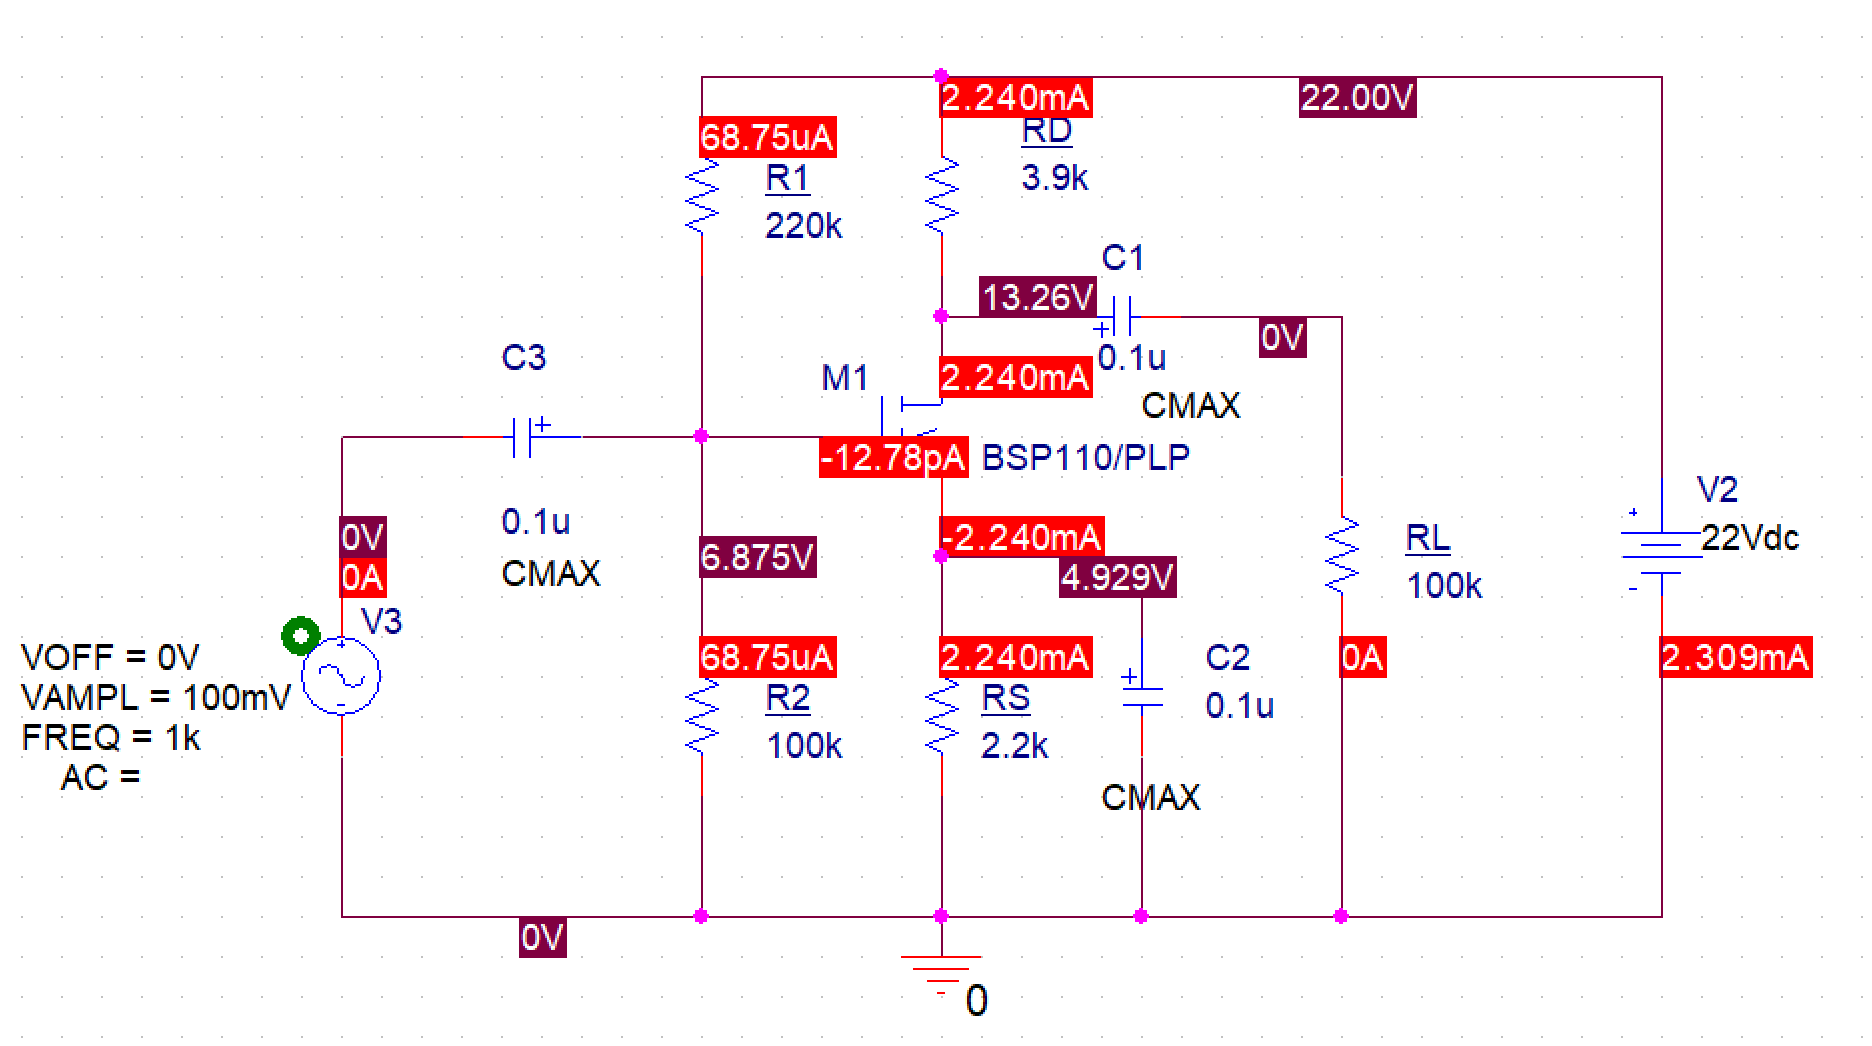
\includegraphics[width=\textwidth]{ECE2200L_Lab8_PSpice.png}
  \caption{PSpice simulation of Step 3 circuit}
  \label{fig:IV2}
\end{figure}

\section*{Conclusion}
As demonstrated above, change in $K_n$ and $V_T$ in a bias circuit designed for a specific MOSFET affects the resulting Q-point parameters.
\end{document}
